%Chapter 4
\chapter{Showcase of Example Unit and Simulation}
\label{chap:simulation}
%
This chapter provides an overview over the developed simulation and what conclusions can be drawn from it.
First a short reasoning for the chosen tool is given.
Then we will introduce a block diagram showing the general approach to the simulation.
This will make the targeted inputs and outputs apparent.
% These parameters are extracted from the \nameref{sec:feasibility} requirements.
Next, models implementing lettuce crop and the technical components specified in the \ref{sub:power-arch} are developed.
The physical environment of the farm is built up to interface with these components.
A first evaluation will be drawn comparing our implementation with state of the art vertical farms.

\section{Introduction to the Simulation Environment}
First a short introduction to Modelica.
% It is an object-oriented language which makes it easy to reuse components.
The language is uniquely catered to describe multi-domain systems.
This is due to its declarative nature.
The equations governing the system at hand are simply written down.
Causality and the progression of the variables over time is taken care of by the solver.
This stands in contrast to imperative languages where a concrete sequence of steps needs to be given.
Not always possible for physical systems.
Matlab Simscape offers similar functionality to integrate with their Simulink program.
But the available libraries are not as vast as for Modelica.
For these reasons Modelica is chosen.
It provides the best framework for our investigation, as our use case is a cyber-physical system.
% It is uniquely suitable for our application -- a cyber-physical system.
% Because we want to simulate a complex cyber-physical system Modelica is chosen.
There exist a variety of GUI-Frontends to the language.
OpenModelica is picked because it is an open-source project freely available.

Additionally, the Modelica Buildings Library is utilized extensively.
It offers a broad range of models specifically for building design.
Questions in this domain are quite similar to the ones posed in this work.
Heat fluxes, solar radiation and mass flows as well as control blocks all have detailed models we can build upon.

\textcolor{Blue}{Intro to the interfaces heat port, real input, fluid port, ...}

\section{Simulation Structure}
% To generate a 
To generate the structure we must first ask: What knowledge shall be gained by the simulation?
This is a question already answered through the \nameref{sec:feasibility} requirements.
The results of this chapter should enable us to make statements about \textit{Energy Consumption}, \textit{Insulation Potential} and \textit{Crop Yield}.
So these are the outputs the simulation shall generate.
Customer acceptance is not part of the technical system and thus not evaluated.
For inputs, we must discern between dynamic and static.
Static data is explained closer in Section \ref{sec:intro-to-models}.

% Next coming back to the architecture, the dynamic variables are the inputs its construction.
Dynamic inputs are the beginning to the simulation flow.
Looking at Figure \ref{fig:system-definition}, any dynamic variable not generated by the farm itself must come from the context.
First the building environment is analyzed.
The property of interest here is the heat flow $\dot{Q}_{\text{FB}}$.
Following the equations from the introduction of \nameref{sub:heat-transfer}, it is calculated with conduction and convection.
As elaborated before radiative heat transfer is investigated separately.
Forced convection is also not applicable here, since there is very little air movement inside buildings.
As a result the only relevant variable is the temperature difference.
% Since air movement inside the building is very little, there is no forced convection.
% And therefore also no dependence on fluid movement ergo air speed.
% It depends upon the air temperature inside the building.
Unfortunately for this study there was no data on the building air temperature to simulate this dynamically.
Consequently, it is assumed to be fixed at \SI{20}{\degreeCelsius} -- normal room temperature.

Next the city environment is broken down.
The natural radiation $R_\text{N}$ is the first dynamic input to the simulation.
Secondly the mass flow $\dot{m}_{\text{Air}}$ is dependent upon air temperature and pressure following the equation in the fundamentals (\ref{sub:ther-props}).
Thirdly heat flow $\dot{Q}_{\text{FC}}$ depends again on temperature difference.
Now forced convection is also taken into account since there is fluid movement in the city environment.
This comes in the form of wind direction and speed.
These values can all be obtained with weather data records for a \ac{tmy}.
% It will be further elaborated upon in the relevant model introduction of Section \ref{sec:intro-to-models}.

% From the outputs and dynamic inputs the general structure of the Simulation is built.
From this, the general simulation flow is developed and shown in Figure \ref{fig:simulation-architecture}.
The left shows the inputs from the weather data.
These are logically grouped into 'Light' for the radiation and 'Air' containing the remainder of the attributes like temperature and wind speed.
Then inside the farm, temperature of the leaf environment is separated out.
The controlled and engineered system are connected together according to our system definition (\ref{fig:system-definition}).
However not all properties shown there need to be evaluated to generate the targeted output.
As shown later in the specific model description only a subset -- shown in the Illustration -- is implemented in the simulation.
The outputs needed to judge feasibility are shown to the right.
% The icons for the different elements are 
The icons used in the diagram are freely available from Google Fonts.
% Freely available Google font icons are used to represent the different blocks in this diagram.
They are also used in the simulation.
\textcolor{Blue}{Envelope is integrated in atmosphere control.}
Same convention as \ref{fig:system-definition} regarding mass, energy and informational flows.
Note that the temperature flow to the plant is informational.
This is no mistake since there is no heat exchange, but only import to the model.

% And so the building and city environment
% our dynamic inputs come from city and building environment.
% In this case they are the weather data providing dry bulb air temperature, natural radiation, wind direction and speed.

% In this section the general approach and architecture of the simulation emerges.
% This follows closely what we have developed so far.
% The system description presented in figure \ref{fig:system-definition} is taken as the physical basis for the models.
% Concrete parameter definitions are taken from the power architecture illustrated in figure \ref{fig:power-architecture}.
% And the output performance indicators are synthesized following the \nameref{sec:feasibility} requirements.

\begin{figure}[htbp]
  \centering
  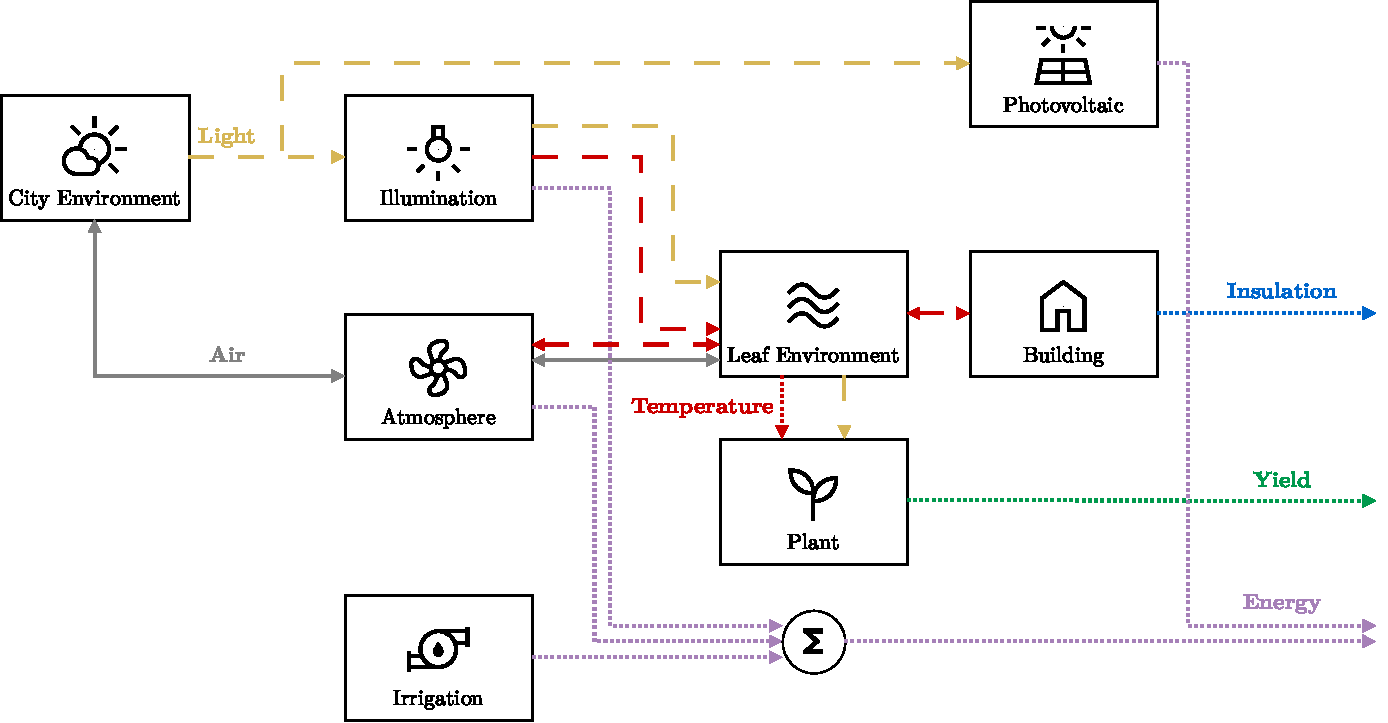
\includegraphics[width=\textwidth]{img/simulation/simulation-architecture.pdf}
  \caption{The simulation architecture implemented to assess the feasibility requirements.}
  \label{fig:simulation-architecture}
\end{figure}

\section{Introduction to the Developed Models}
\label{sec:intro-to-models}
\textcolor{Blue}{List static variables?}

% Static variables are things which can be build right into the models as parameters.
Modelica is object-oriented, which enables the construction of a general model with parameters.
These are then instantiated and the specific values for different entities can be put in.
Examples for our application include the orientation of the building walls or the optimal \ac{dli} for the chosen crop.
The static inputs of each model will be listed in their presentation in Section \ref{sec:intro-to-models}.
% These are for example the orientation of the building, optimal \ac{dli} for the plant
\textcolor{Blue}{Capitalize Figure, Section and so on in the rest of the thesis.}
Introduce that there are four farms.

The introduction of the models follows a pattern.
First the models and their static parameters are established and then the dynamic inputs and outputs are listed.

We follow the same order as introduced in the \ref{sec:system-analysis} first describing the plant and its environments, then the engineered systems and lastly implementing the context.

\subsection{Geometric Calculations}
depth of the farm  window width height of the building
Geometric calculations!
Do a table with these.

\subsection{Plant Model}

\subsubsection{Yield}
\label{subsub:yield-model}
The yield model employed in this study is a system of two \acp{ode}.
It was developed by @van\_henten1994 and uses dry weight to assess the growth of lettuce.
For this, mass is split up into the state variables structural dry weight $x_{\text{sdw}}$ (\si{\g\per\square\m}) and non-structural dry weight $x_{\text{nsdw}}$ (\si{\g\per\square\m}).
% The model is composed of two nonlinear ordinary differential equations.
The development of these two state variables over time is given by
\begin{align*}
  % \begin{equation*}
  \frac{\mathrm{d}x_{\text{nsdw}}}{\mathrm{d}t} &= c_\alpha f_{\text{phot}} - r_{\text{gr}} x_{\text{sdw}} - f_{\text{resp}} - \frac{1-c_\beta}{c_\beta} r_{\text{gr}} x_{\text{sdw}}\\
  % \end{equation*}
  % \begin{equation*}
  \frac{\mathrm{d}x_{\text{sdw}}}{\mathrm{d}t} &= r_{\text{gr}} x_{\text{sdw}}
  % \end{equation*}
\end{align*}
with parameters $c_\alpha$ (-) being the conversion rate of CO$_2$ to CH$_2$O and $c_\beta$ (-) representing the yield factor.
$f_{\text{phot}}$ (\si{\g\per\square\m\per\s}) describes gross canopy photosynthesis, $f_{\text{resp}}$ (\si{\g\per\square\m\per\s}) the maintenance respiration and $r_{\text{gr}}$ (\si{\per\s}) the specific growth rate.

Which themselves are given by
\begin{align*}
  r_{\text{gr}} &= c_{\text{gr,max}} \frac{x_{\text{nsdw}}}{c_\gamma x_{\text{sdw}} + x_{\text{nsdw}}} {c_{\text{Q10,gr}}}^{(u_\text{T}-20)/10}\\
  \\
  f_{\text{resp}} &= (c_{\text{resp,sht}}(1-c_\tau)x_{\text{sdw}}+c_{\text{resp,rt}}c_\tau x_{\text{sdw}}) {c_{\text{Q10,resp}}}^{(u_\text{T}-25)/10}\\
  f_{\text{phot}} &= (1-\exp(-c_\text{K} c_{\text{lar}} (1-c_\tau) x_{\text{sdw}})) f_{\text{phot,max}}
\end{align*}
with $c_{\text{gr,max}}$, $c_\gamma$, $c_{\text{Q10,gr}}$, $c_{\text{resp,sht}}$, $c_\tau$, $c_{\text{resp,rt}}$, $c_{\text{Q10,resp}}$, $c_\text{K}$ and $c_{\text{lar}}$ all being constants specific to lettuce.
A clear overview over these static values and their biological meaning can be found in @abedi2023 or in the original paper @van\_henten1994.
The air temperature $u_\text{T}$ (\si{\degreeCelsius}) is the first dynamic input to this model.

Next the gross carbon dioxide assimilation rate $f_{\text{phot,max}}$ (\si{\g\per\square\m\per\s}) can be calculated with
\begin{align*}
  f_{\text{phot,max}} &= \frac{\epsilon u_{\text{par}} g_{\text{CO}_2} c_\omega (u_{\text{CO}_2} -\Gamma)}{\epsilon u_{\text{par}} + g_{\text{CO}_2} c_\omega (u_{\text{CO}_2} -\Gamma)}\\
  \epsilon &= c_\epsilon \frac{u_{\text{CO}_2} - \Gamma}{u_{\text{CO}_2} + 2\Gamma}\\
  \Gamma &= c_\Gamma {c_{\text{Q10,}\Gamma}}^{(u_\text{T}-20)/10}\\
  g_{\text{CO}_2} &= \left(\frac{1}{g_{\text{bnd}}} + \frac{1}{g_{\text{stm}}} + \frac{1}{g_{\text{car}}}\right)^{-1}\\
  g_{\text{car}} &= -1.32 \cdot 10^{-5} \si{\m\per\s\per\square\degreeCelsius} {u_\text{T}}^2 + 5.94 \cdot 10^{-4} \si{\m\per\s\per\degreeCelsius} u_\text{T} - 2.64 \cdot 10^{-3} \si{\m\per\s}
\end{align*}
where $c_\omega$, $c_\epsilon$, $c_\Gamma$, $c_{\text{Q10,}\Gamma}$, $g_{\text{bnd}}$ and $g_{\text{stm}}$ again are constant coefficients.
Interesting for us are the two other dynamic inputs, the incident \ac{par} $u_\text{par}$ (\si{\W\per\square\m}) and the CO$_2$ concentration $u_{\text{CO}_2}$ (\si{\ppm}).
These calculations are implemented into a Modelica model as can be seen in Listing \ref{lst:yield}.

%[language=modelica, basicstyle=\fontsize{9pt}{10.5pt}\ttfamily]
\begin{lstlisting}[basicstyle=\fontsize{9pt}{10.5pt}\ttfamily, caption={Modelica model for lettuce yields per \si{\square\m}}, label=lst:yield]
model plant_yield
  /*
    input, output and variable definition skipped for readability
  */

initial equation
  x_nsdw = x_nsdw_start;
  x_sdw = x_sdw_start;

equation
  when reset then
    reinit(x_nsdw, x_nsdw_start);
    reinit(x_sdw, x_sdw_start);
  end when;

  der(x_nsdw) = c_alpha*f_phot - r_gr*x_sdw - f_resp - ((1 - c_beta)/c_beta)*r_gr*x_sdw;
  der(x_sdw) = r_gr*x_sdw;

  r_gr = c_gr_max*(x_nsdw/(c_gamma*x_sdw + x_nsdw))*c_q_10_gr^(((air_temperature - 273.15) - 20)/10);
  f_resp = (c_resp_sht*(1 - c_tau)*x_sdw + c_resp_rt*c_tau*x_sdw)*c_q_10_resp^(((air_temperature - 273.15) - 25)/10);
  f_phot = (1 - exp(-c_k*c_lar*(1 - c_tau)*x_sdw))*f_phot_max;

  f_phot_max = (epsilon*par*g_co2*c_omega*(co2_concentration - capital_gamma))/(epsilon*par + g_co2*c_omega*(co2_concentration - capital_gamma));
  capital_gamma = c_cap_gamma*c_q_10_cap_gamma^(((air_temperature - 273.15) - 20)/10);
  epsilon = c_epsilon*(co2_concentration - capital_gamma)/(co2_concentration + 2*capital_gamma);
  g_co2 = 1/((1/g_bnd) + (1/g_stm) + (1/g_car));
  g_car = max(-1.32e-5*(air_temperature - 273.15)^2 + 5.94e-4*(air_temperature - 273.15) - 2.64e-3, Modelica.Constants.small);

  dw = a_plant*(x_nsdw + x_sdw) / 1000;
end plant_yield;
\end{lstlisting}

There are some notable differences to the original equations.
Temperature in Modelica is given in Kelvin and thus $u_\text{T}$ needs to be converted before it can be used in the calculation.
% The air temperature $u_\text{T}$ is calculated in Kelvin in Modelica and so needs to be converted to \si{\degreeCelsius} as can be seen for instance in line 16.
A reset is implemented in lines 11 to 14 to simulate a harvest.
After which the state variables are reinitialized with their start values.
This initial condition was matched to the original paper specifying \SI{75}{\percent} structural and \SI{25}{\percent} non-structural weight for the planting stage.
Their total dry weight for the young plants ranged from 0.72 to \SI{2.7}{\g\per\square\m} for greenhouse cultivation.
The upper end of this spectrum is implemented in the model since hydroponic cultivation allows for high plant densities.
Another difference is that the irradiance $u_{\text{par}}$ is going into the equation with the unit \si{\W\per\square\m}.
So the total \ac{par} in \si{\umol\per\square\m\per\s} is divided by the conversion factor \SI{4.56}{\umol\per\W\per\s} to get the equivalent value in \si{\W\per\square\m} @reis2020.
The equation for $g_\text{car}$ is a quadratic polynomial with roots at \SI{5}{\degreeCelsius} and \SI{40}{\degreeCelsius}.
To avoid a division by zero it is wrapped in the \lstinline{max()} function and compared with \lstinline{Modelica.Constants.small}.

The model implementation was validated following a similar setup as the original paper.
Their input data was not available, but was approximated with similar weather data from Germany.
This resulted in an output close to the one observed in @van\_henten1994.

From the two \acp{ode} we can extract the \textit{Dynamic Inputs}.
These are the air temperature $T$, the \ac{par} $R_\text{T}$ and the carbon dioxide concentration.
As we do not have information on the CO$_2$ from the weather data or air volume inside the farm it is fixed to \SI{417}{\ppm} -- a recent value from 2022 according to https://doi.org/10.56028/aetr.4.1.470.2023.
The \textit{Output} of the model are the two state variables describing the dry weight.
Since they do not need to be differentiated in the further investigation, they are added together to obtain the total dry weight $\text{dw} = (x_\text{nsdw} + x_\text{sdw}) / 1000$ in \si{\kg\per\square\m}.

\subsubsection{Evapotranspiration}
An implementation of a model for lettuce evapotranspiration is available in the plant definition.
It is based on the Penman–Monteith equation with crop coefficients from @lópez\_mora2024.
But it yielded unrealistically high results.
The source of this inconsistency was not further investigated, since irrigation is no focus in this study.
Instead, a pessimistic assumption on the water use was made to dimension the water pump and judge its energy consumption.
It still shows inconsequential power draw in comparison to the lighting system.

% \pagebreak

\subsection{Leaf Environment}
\begin{wrapfigure}{R}{0.3\textwidth}
    \centering
	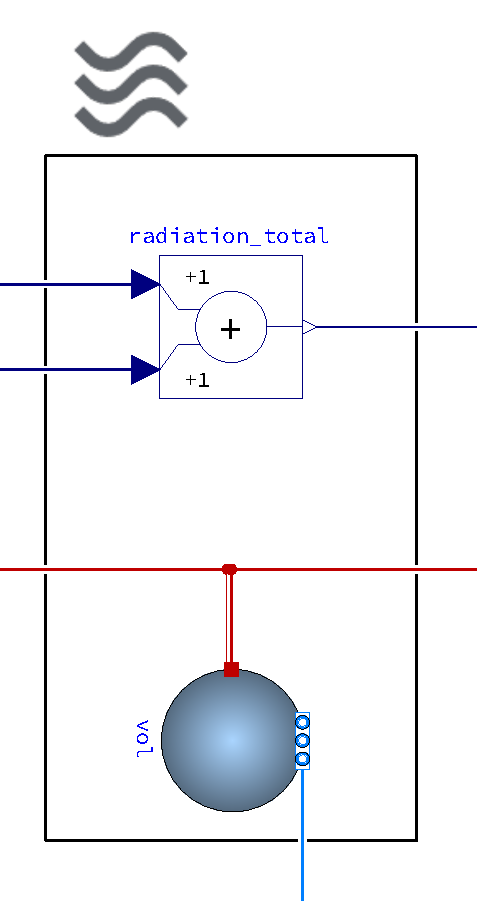
\includegraphics[width=0.25\textwidth]{img/simulation/leaf-env.pdf}
	\caption{The leaf environment in the simulation.}
	\label{wfig:leaf-env}
\end{wrapfigure} 

The leaf environment simply consists of a summation to calculate the total radiation from natural and artificial sources as well as the model \lstinline{Buildings.Fluid.MixingVolumes.MixingVolume}.
The mixing volume requires three static inputs.
A fluid definition, the volume size and the nominal mass flow.
The fluid is taken to be  \lstinline{Buildings.Media.Air "Moist air"} -- the standard air environment following the documentation of the Modelica Building library.
The volume is passed along to be defined later in the north-east, north-west, south-west and south-east facing instances.
Respective for the four sides of the building.
The nominal mass flow depends on the rest of the implementation.
Not too much thought is given here since according to the documentation, it is mostly used for numerical robustness.
It is set to a small value now and later filled in with the average of the maximum air flow for the four farms of around \SI{90}{\kg\per\s}.
The 'radiation\_total' block takes the shaded plus artificial radiation $R_\text{S} + R_\text{A}$ as \textit{Dynamic Inputs} and \textit{outputs} the total irradiance $R_\text{T}$.
For the mass and heat flows there can be no definition of input and output since the flow direction is dynamically calculated by the simulation.

The mixing volume model is also able to handle trace substances like water and CO$_2$.
This is not used in our implementation but offers possibilities to simulate humidity and elevated carbon dioxide levels in the future.
% can also track trace substances like water and co2 so can be further built upon in future studies.

\subsection{Illumination}
Now that the relevant parts of the controlled system are implemented, we can look at the engineered system.
First the illumination control is modeled.
For this the natural radiation is needed as a control signal.
Conveniently there are already models implemented, computing the components for direct and diffuse radiance from the weather data.
The ground reflected radiation is part of the diffuse irradiance in this context.
These models as well as the 'weaBus' carrying the weather data can be seen on the left of the shading model in Figure \ref{fig:shading}.
The surface tilt and azimuth are taken as static parameters by these blocks.
Tilt is set to \SI{90}{\degree} as the farm is placed on the side of a building.
The azimuth is passed along to the instance definition respective the orientation of the building face the farm is mounted to.
Additionally, the 'HDifTilIso' model can define the ground reflectance.
This is left at the standard value of the model definition which is 0.2.

\subsubsection{Shading}
With the natural radiation taken care of, the awning is examined more closely.
Shading cloths for greenhouses are usually chosen by their diffusion percentage.
That is the proportion of light which will not pass through.
They are available in a range from 20 up to \SI{80}{\percent} diffusion.
An industry standard shading cloth with \SI{40}{\percent} is chosen as Germany does not experience extreme levels of irradiance.
As such the awning extending the fabric is simply modeled as a multiplication block governed by a P controller.
The controller is limited from the values 0.6 to 1.
Effectively letting 60 to \SI{100}{\percent} of the natural radiation pass into the farm according to the incident intensity.
Lettuce experiences light stress above \SI{290}{\umol\per\square\m\per\s} and so the light set point is determined to be at this value @chen2022.
The output of the shade block is multiplied by \SI{2.02}{\umol\per\W\per\s} to get \ac{par} from the suns' radiation @reis2020.
This is then fed back to the P controller.
Notice that the conversion factor at this point is different from the one used in the plant model.
This is because here we are converting full spectrum light to the photosynthetic relevant range from 400 to \SI{700}{\nm}.
With the plant model input, we already had this range given and just wanted to exchange the units.

Natural irradiance $R_\text{N}$ contained in the weather data is the \textit{Dynamic Input} for the block.
The \textit{Output} is the shaded radiance $R_\text{S}$.

\begin{figure}[htbp]
  \centering
  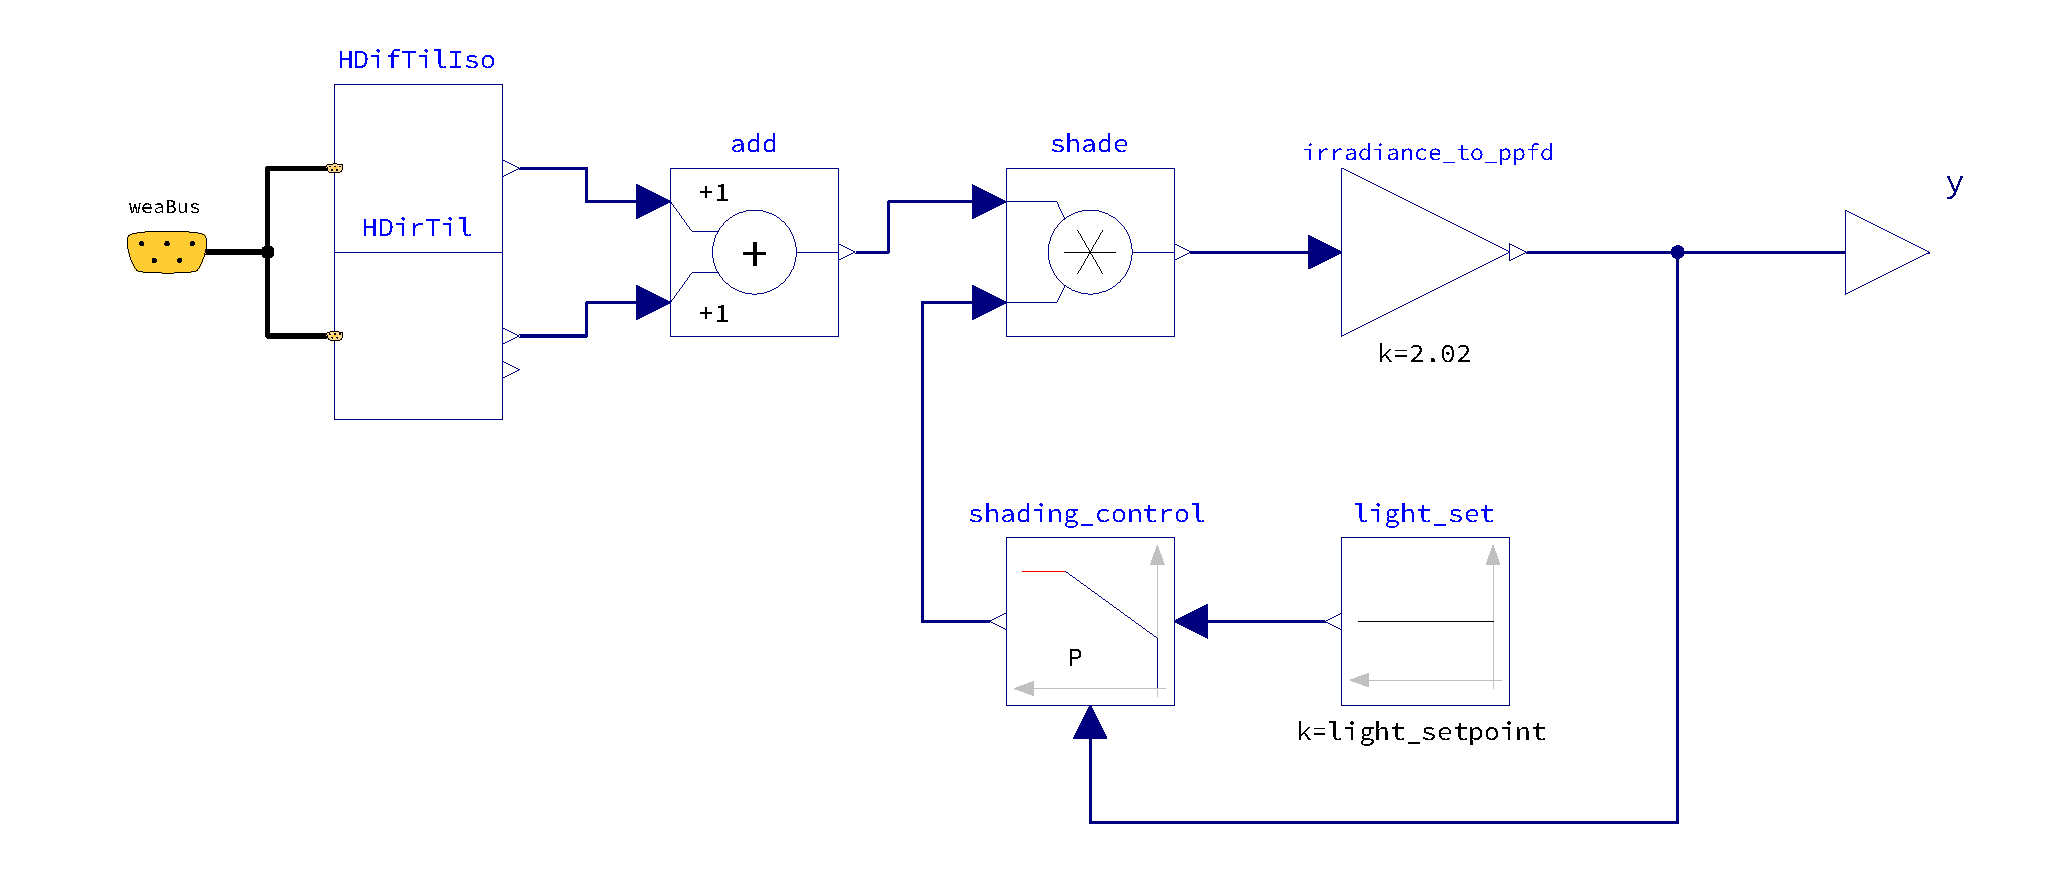
\includegraphics[width=\textwidth]{img/simulation/shading.pdf}
  \caption{The model calculating the shaded irradiance.}
  \label{fig:shading}
\end{figure}

% https://www.growerssupply.com/prod/gs-reflective-shade/pgshadercus.html

\subsubsection{\ac{led}}
The \ac{led} model now takes the shaded radiation and calculates the \ac{dli} for it.
This is done by an integration block with a daily reset.
Then the signal is sampled at the end of each day and subtracted from the optimal \ac{dli}.
Which is \SI{14.4}{\mol\per\square\m\per\day} for lettuce according to @pennisi2020.
As sometimes the actual irradiance will be above the optimal value, a limiter rectifies the signal.
This is to remove nonsensical negative values.
As we can not take light away with the \acp{led}.
Then the time to achieve optimal \ac{dli} is calculated with the actual \ac{ppfd} output of the lighting system.
The chosen \acp{led} were already introduced in Section \ref{sub:power-arch}.
Their light flux is \SI{218.28}{\umol\per\square\m\per\s}.
Time to achieve optimal \ac{dli} is calculated and compared to a timer.
It is started every day if supplemental lighting is needed.
A simple on/off controller then switches on for the requested time interval.

This enables the \textit{Outputs} 'ppfd\_out' and generated waste heat at the red heat port.
$R_\text{A}$ and $\dot{Q}_\text{R}$ respectively in the system definition (\ref{fig:system-definition}).
Waste heat is calculated from the efficiency of \SI{62.2}{\percent} for the chosen light fixture.
Also, the total power output is given.
For this the power draw per square meter of \SI{77.76}{\W} is multiplied by the growing area.
This area is defined later in the relevant instances.
The \textit{Dynamic Input} as discussed before is the shaded radiation $R_\text{S}$.

Note that this control waits until the end of the day to calculate the missing \ac{dli}.
As such it turns on at 00:00 the next day and illuminates during nighttime.
This might be good behavior considering electricity prices, but is not applicable everywhere.
For instance if the system is installed at residential buildings, inhabitants would not want to be illuminated during sleeping hours.
In this work no time optimal control for the lighting system is considered.
Only optimality regarding the total irradiance is aimed for.

\begin{figure}[htbp]
  \centering
  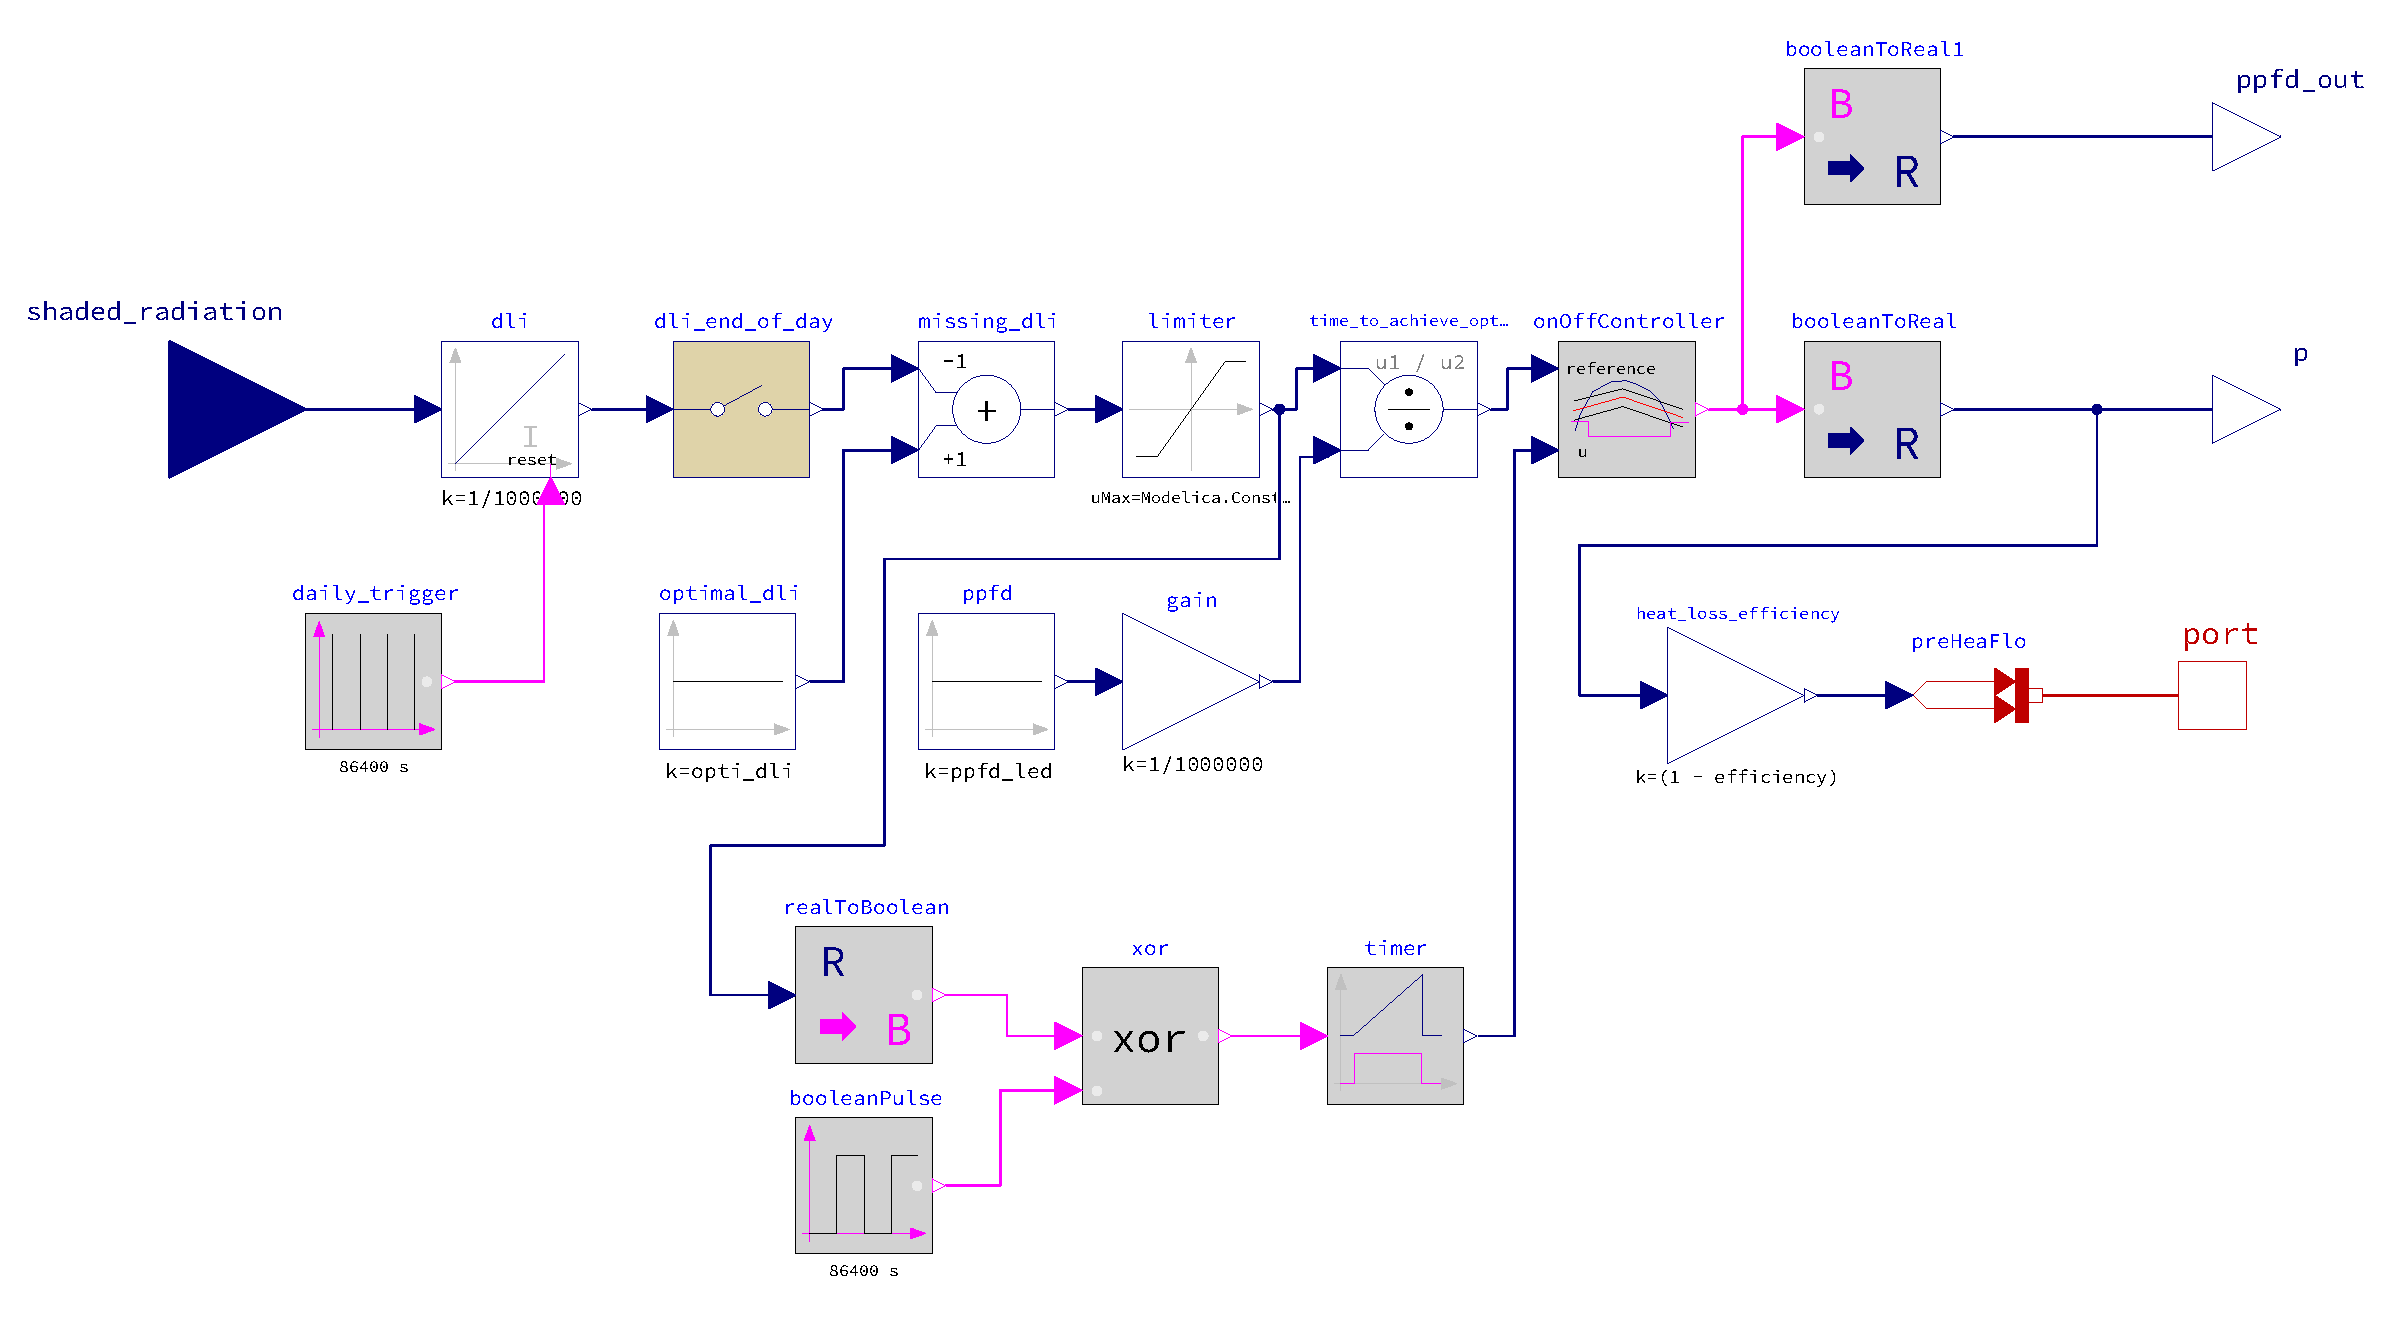
\includegraphics[width=\textwidth]{img/simulation/led.pdf}
  \caption{The \ac{led} model and control circuitry.}
  \label{fig:led}
\end{figure}

The model was verified by visually inspecting the output as can be seen exemplary in Figure \ref{fig:led-validation}.
On the first day (\SI{4.85}{\mega\s} - \SI{4.92}{\mega\s}) the incident radiation (red) is high with a resulting \ac{dli} of \SI{17.48}{\mol\per\square\m\per\day}.
Consequently, the supplemental lighting (blue) is not turned on.
The second day shows less natural light (\SI{13.21}{\mol\per\square\m\per\day}) and therefore the \acp{led} are turned on at 00:00 (\SI{5.01}{\mega\s}) the next day.
The third day (\SI{5.01}{\mega\s} - \SI{5.1}{\mega\s}) is quite cloudy, hence the artificial light is turned on for longer.
This also highlights the non-optimality of the timing as it illuminates into the sunrise of the next day.
A smarter lighting system can be the grounds for further research.

\begin{figure}[htbp]
  \centering
  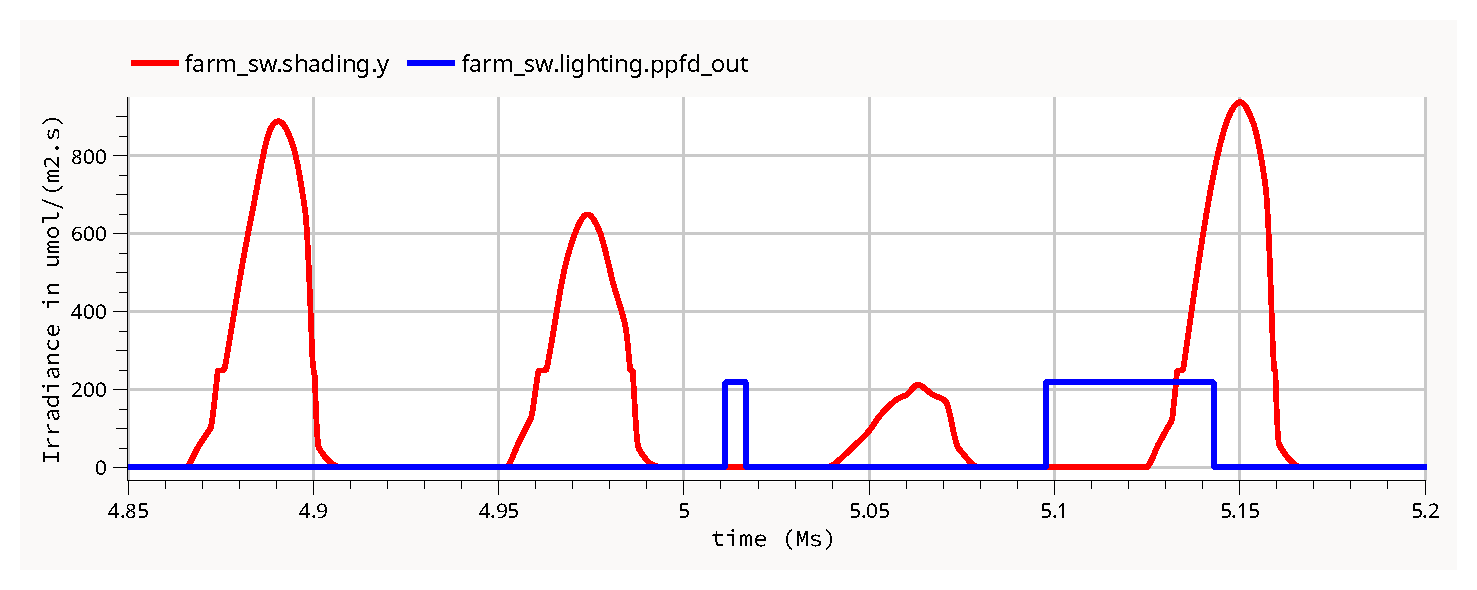
\includegraphics[width=\textwidth]{img/simulation/led-validation.pdf}
  \caption{\ac{led} model validation.}
  \label{fig:led-validation}
\end{figure}

\subsection{Atmosphere}
\subsubsection{Envelope}
For the simulation of the atmosphere control, we also consider the envelope.
The model for its heat transfer is introduced in Figure \ref{fig:envelope}.
Weather information is again carried by the weather bus.
It is used in 'pre\_tem' to prescribe the outside temperature onto the heat port of the convection component.
Wind direction and speed is also taken from the weather data and fed to 'conv\_out'.
The component takes the area over which the convection is happening, the roughness of the solid material, the azimuth and the tilt as input.
The area and azimuth are again passed to the later instances.
Since the envelope is made of glass, the roughness is set to \lstinline{SurfaceRoughness.VerySmooth}, following the documentation.
Tilt is fixed at \SI{90}{\degree}.
Next the data record 'glass' can be seen in the bottom of the model.
It was taken from the Buildings library with the thickness parameter adjusted to \SI{5}{\mm}.
This material definition as well as the envelope area are passed to the 'conduction' component.
Then the convection facing the farms' interior is connected to the aptly named heat port.
When specifying the air direction for forced convection, we have to be thorough.
Usually for weather data it is given as a cardinal direction.
However, air flow in our farm will be mostly upwards.
Checking in the model the forced convection coefficient $h_\text{f}$ is calculated with $W=1$ for windward surfaces and $W=0.5$ for leeward surfaces.
There is no further distinction made.
A \SI{90}{\degree} flow along the surface is considered windward in the documentation and as such the value $W=1$ is applicable for upwards air movement.
So the constant $\pi - \text{azimuth}$ is fed to the component as the air direction, insuring it is normal on the surface.
The air speed is calculated from the fluid flow in the farm and input here.
Heat gain from solar radiation is considered as well.
For this the shaded radiation is multiplied by the solar heat gain coefficient.
Its value for windows is typically in the range of 0.2 to 0.7 according to the British Fenestration Rating Council.
A value of 0.5 is used in our simulation.

With this we have defined the \textit{Inputs} as the shaded radiation $R_\text{S}$, air speed inside the farm and weather information.
The \textit{Output} is heat flow information.

% Wind direction for forced convection exterior.
% It is calculated with W=1 for windward surfaces and W=0.5 for leeward surfaces.
% @Buildings.HeatTransfer.Convection.Exterior.
% So any wind direction into the surface will result in the expected behavior.

\begin{figure}[htbp]
  \centering
  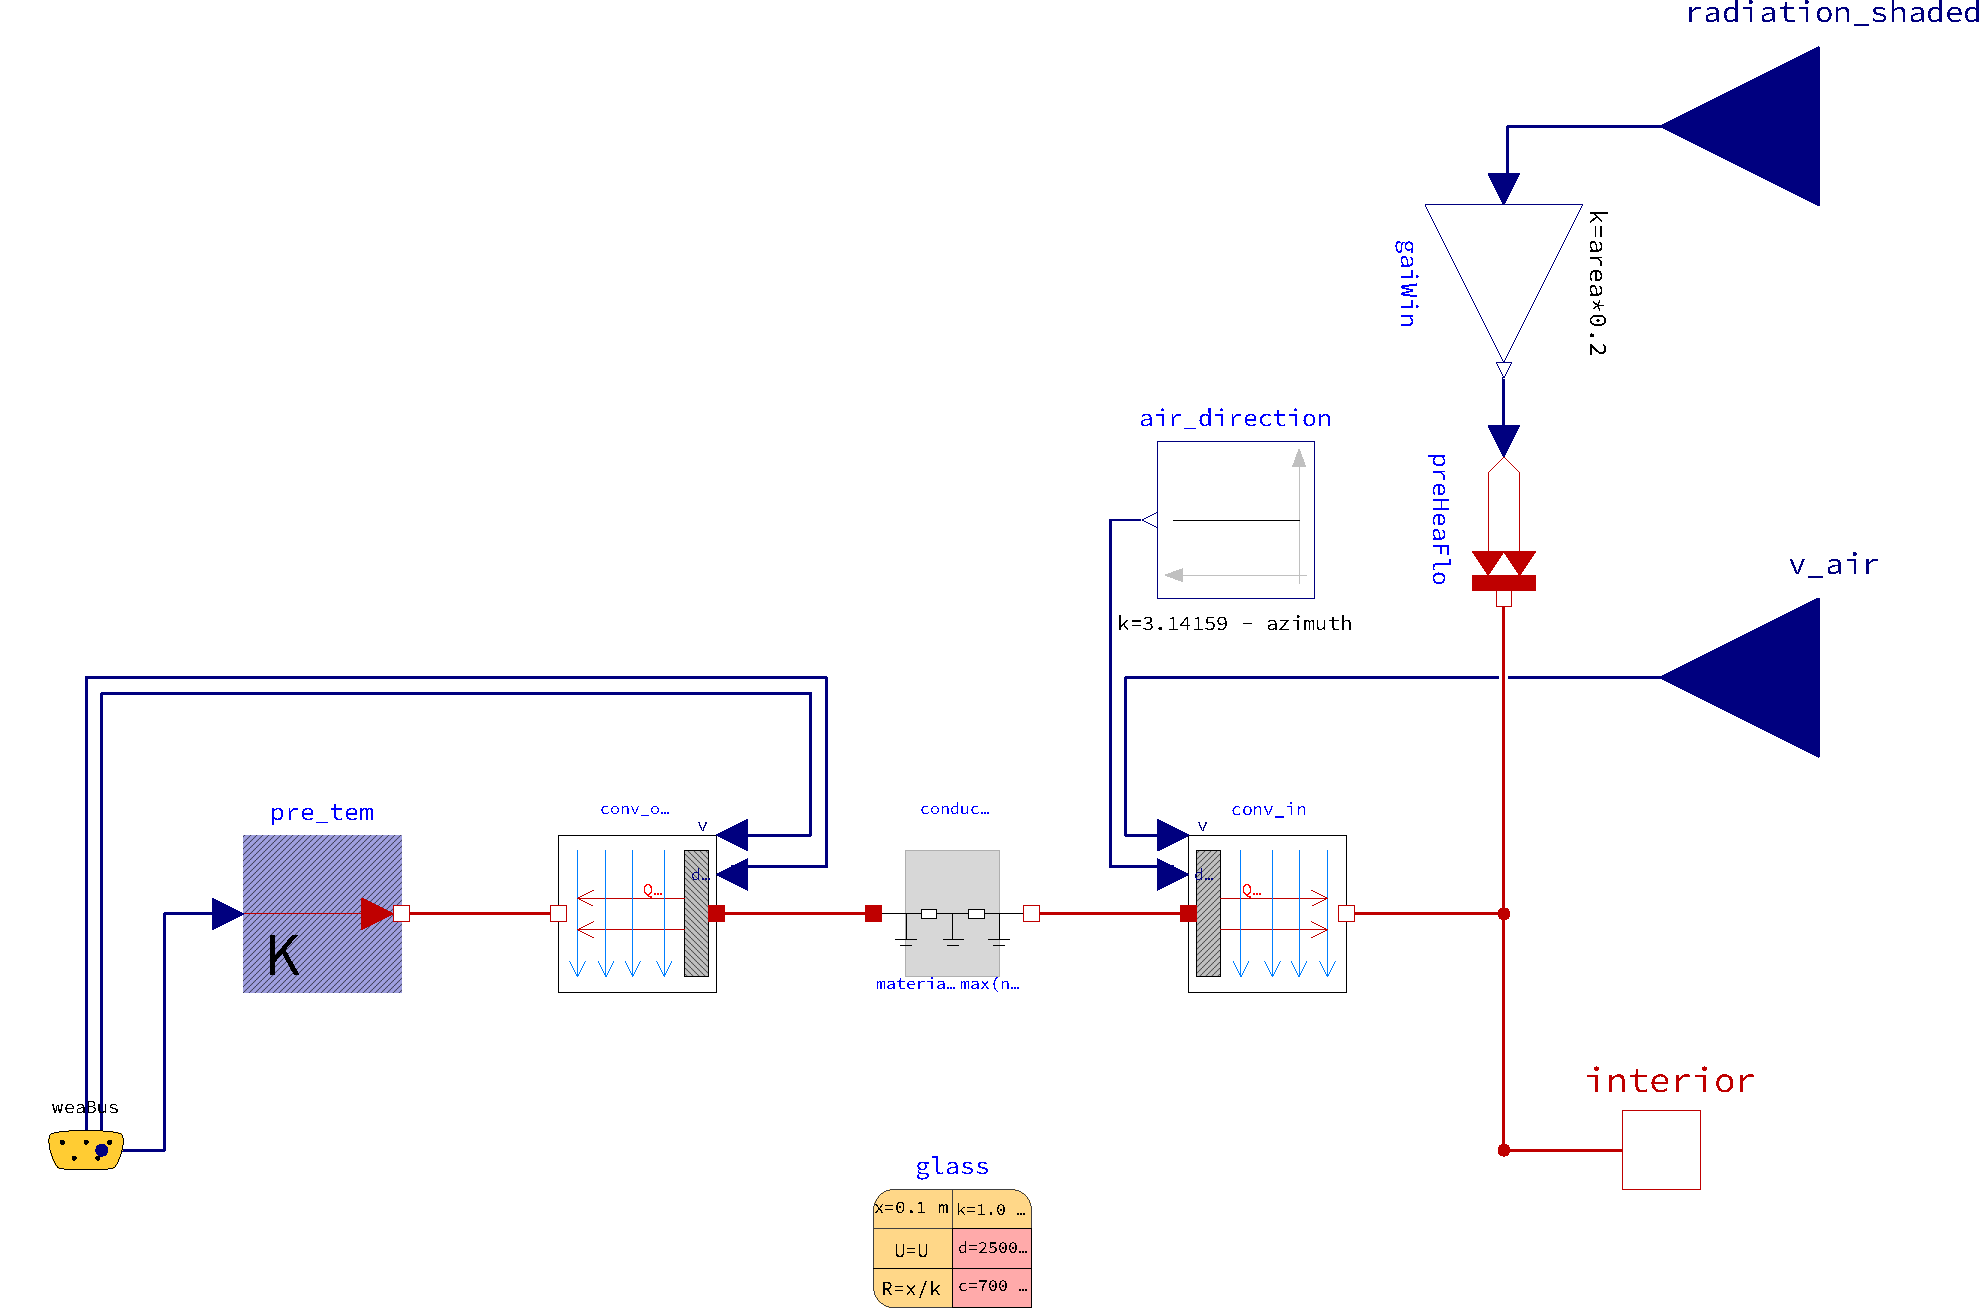
\includegraphics[width=\textwidth]{img/simulation/envelope.pdf}
  \caption{The heat transfer model of the envelope surrounding the farm.}
  \label{fig:envelope}
\end{figure}


\subsubsection{Air Control}
\begin{wrapfigure}{R}{0.65\textwidth}
    \centering
	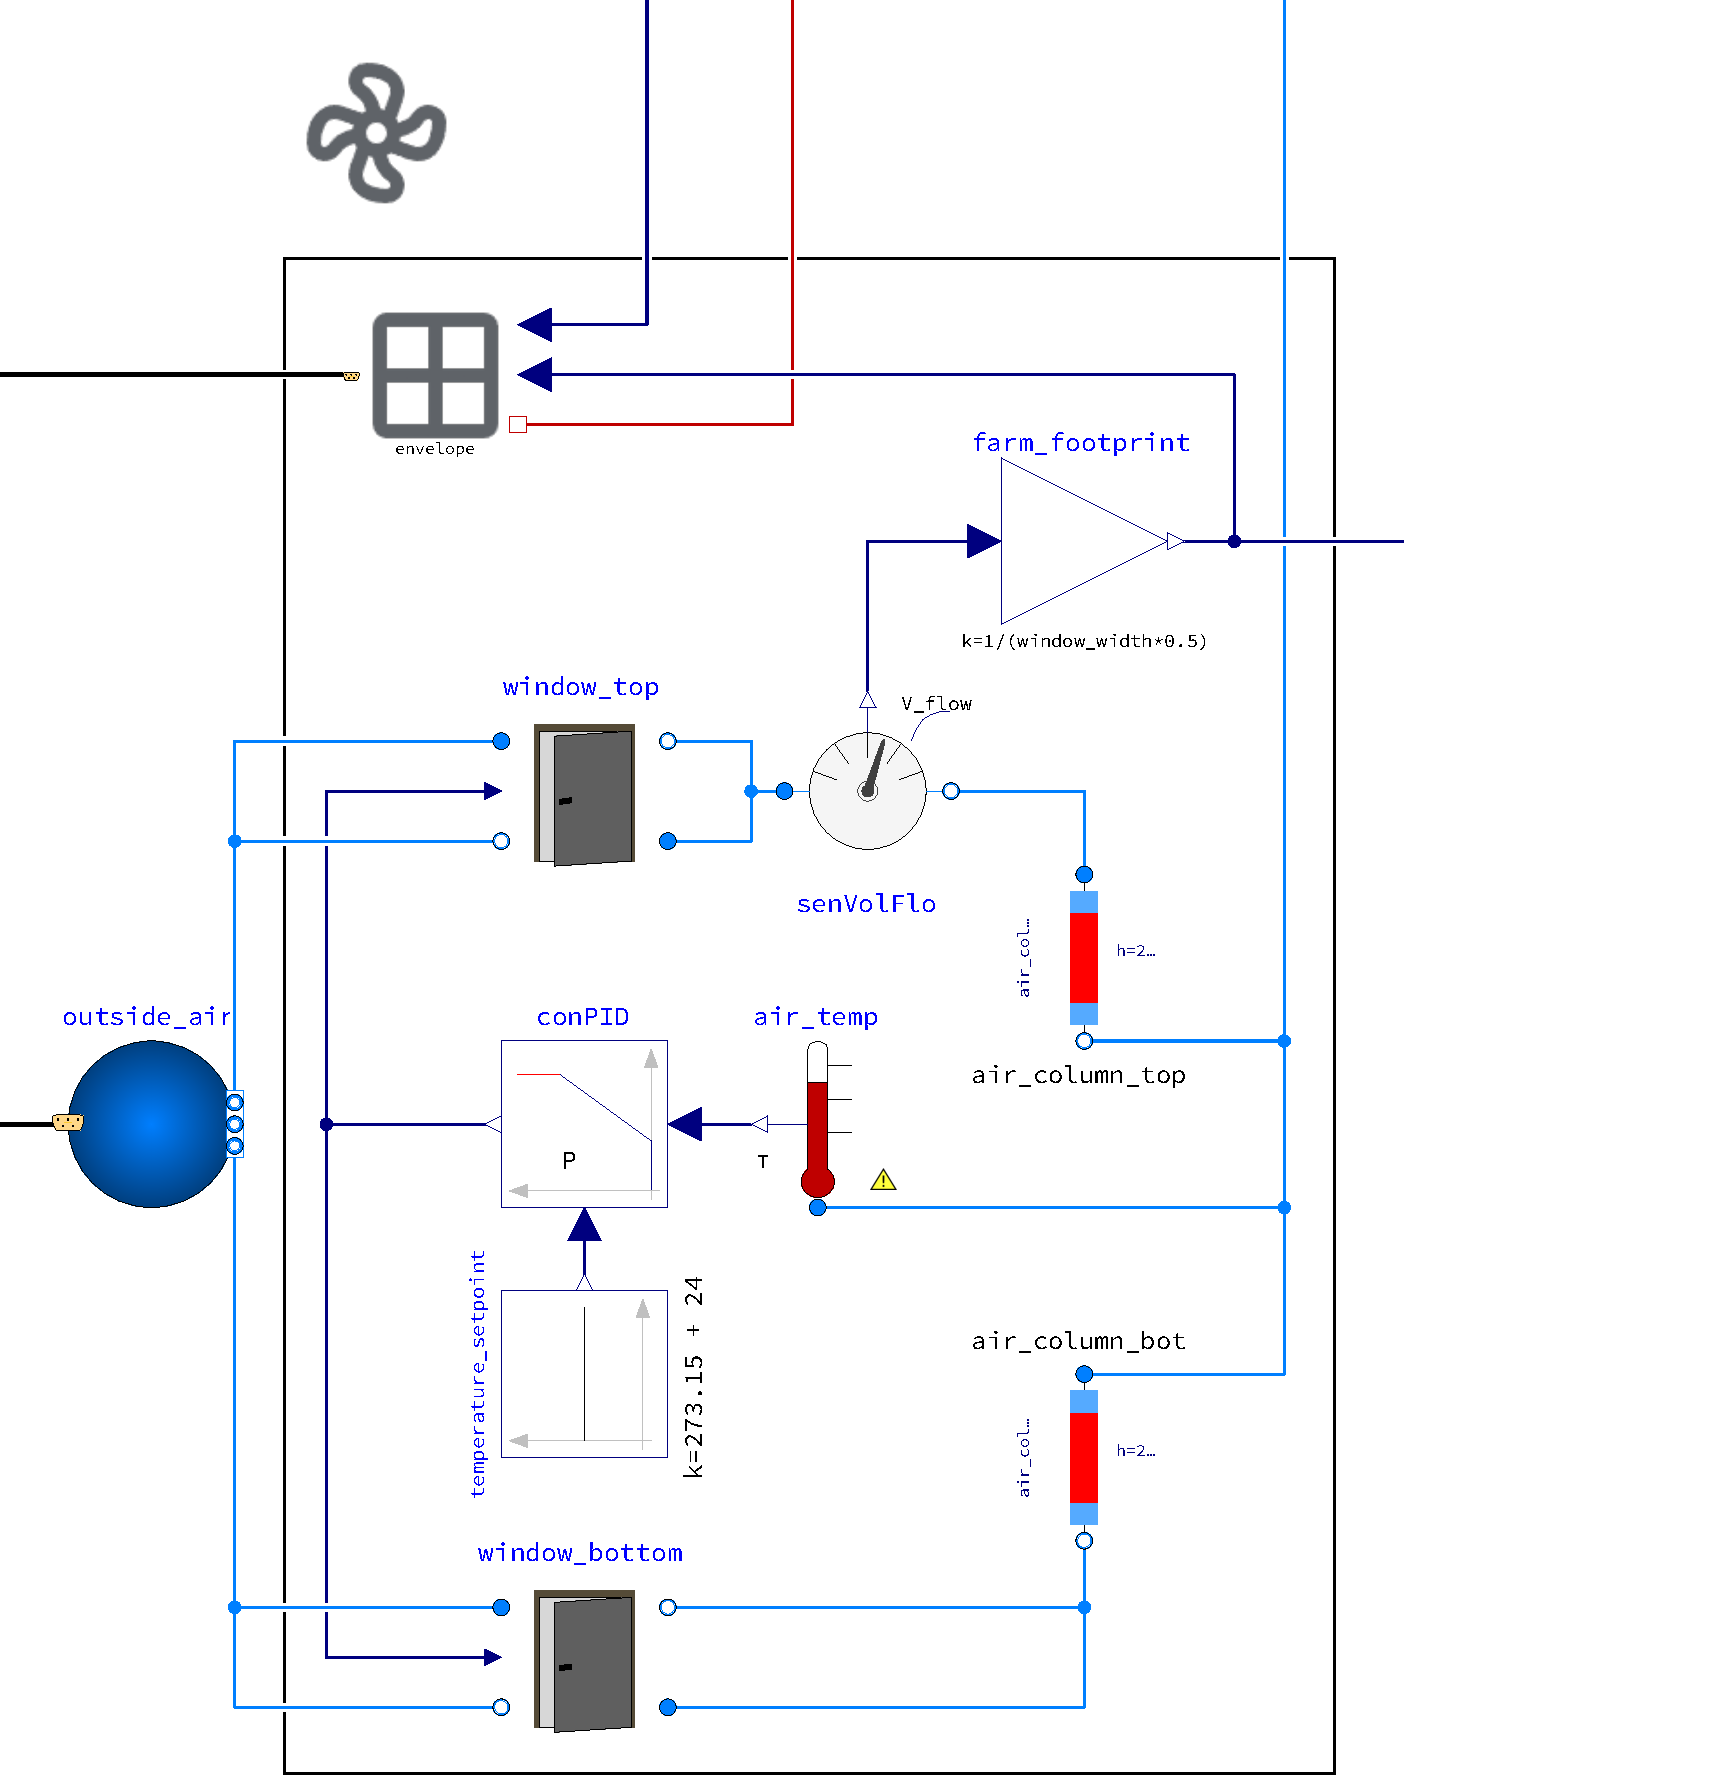
\includegraphics[width=0.6\textwidth]{img/simulation/atmosphere.pdf}
	\caption{The atmosphere control.}
	\label{wfig:atmosphere}
\end{wrapfigure} 

As elaborated previously the atmosphere control in our concept consists of simple controlled windows.
The windows are modeled with \lstinline{Buildings.Airflow.Multizone.DoorOperable}.
At first glance it seems odd to take a door model for the implementation of windows.
However, it is a "Model for bi-directional air flow through a large opening such as a door which can be opened or closed based on the control input signal y", according to the documentation \textcolor{Blue}{needs ref}.
Which tells us it can also be used to model a window like opening.
No more appropriate model was found by the author in the library.
The equation governing the volume flow rate of air for the closed opening is given by
$$
\dot{V}_\text{closed} = c_\text{closed} \Delta p ^ {m_\text{closed}}
$$
with $c_\text{closed}$ being the flow coefficient and $m_text{closed}$ the flow exponent \textcolor{Blue}{needs ref}.
This computes air flow through inevitable small gaps.
The values for these coefficients were left at the default for the model.
The volume flow rate for the open window $\dot{V}_\text{open}$ is given by the equation introduced in the fundamentals (\ref{sub:ther-props}).
The total air flow resulting from the operation of the opening is calculated with
$$
\dot{V}_\text{total} = (y-1)\dot{V}_\text{closed} + y \dot{V}_\text{open}
$$
according to the documentation of the model, where $y$ is the control signal.
These models need geometric information to go off of.
The height of the window was fixed to \SI{0.4}{\m}.
The widths of the single windows is added together and assumed to be equal to the breadth of the farm.
 % and is passed along to the instance definition.
% This describes the total window area, of course it would be unfeasible to have one 
These dimensions ensured sufficient air flow in summer temperatures.
The area of the gaps specifying the closed window was set to \SI{0.001}{\square\m}.
A small value, since we would want to have small gaps for the windows, to not allow unwanted airflow.

The actual pressure difference $\Delta p$ needed to calculate the air flow is given by the components 'air\_column\_top' and 'air\_column\_bot'.
Its calculation was already introduced in Section \ref{sub:ther-props}.
With \SI{11.25}{\m} being the height of the two air columns respectively.
That is half the height of the building.
The geometric calculations are introduced later in the instance definitions.

From this volume flow through the farm, also the air speed is calculated with $v_\text{air} = \dot{V}_\text{total}\, / \, A_\text{footprint}$.
The footprint area takes the window width and depth of the farm of \SI{0.5}{\m} into account $A_\text{footprint} = w_\text{window} * d_\text{farm}$.

Control of the windows is taken over by a simple P controller.
Its set point is fixed to \SI{24}{\degreeCelsius}, the optimal temperature for lettuce growth following \textcolor{Blue}{needs ref}.

Next the power consumption is evaluated in Figure \ref{fig:window-motors}.
But how do we model this?
The motors actuating the windows are active when there is a change of the control signal.
So to get this information, the derivative is taken.
This makes sense as it is higher when there is more change.
Then the absolute value is computed and compared to a threshold value.
This is needed since we do not have to actuate the motors for any miniscule change.
An on / off controller then turns the motors on when the threshold is passed.
The value for this boundary is taken from the simulation data.
No extensive analysis is taken here, since the resulting power consumption is mostly negligible.
The chosen motors introduced in \ref{sub:power-arch} have a wattage of \SI{26}{\W}.
As argued before, two of them are deployed.
So the output of the controller is multiplied with \SI{52}{\W} in the 'booleanToReal' block.

Inputs and Outputs.

\begin{figure}[htbp]
  \centering
  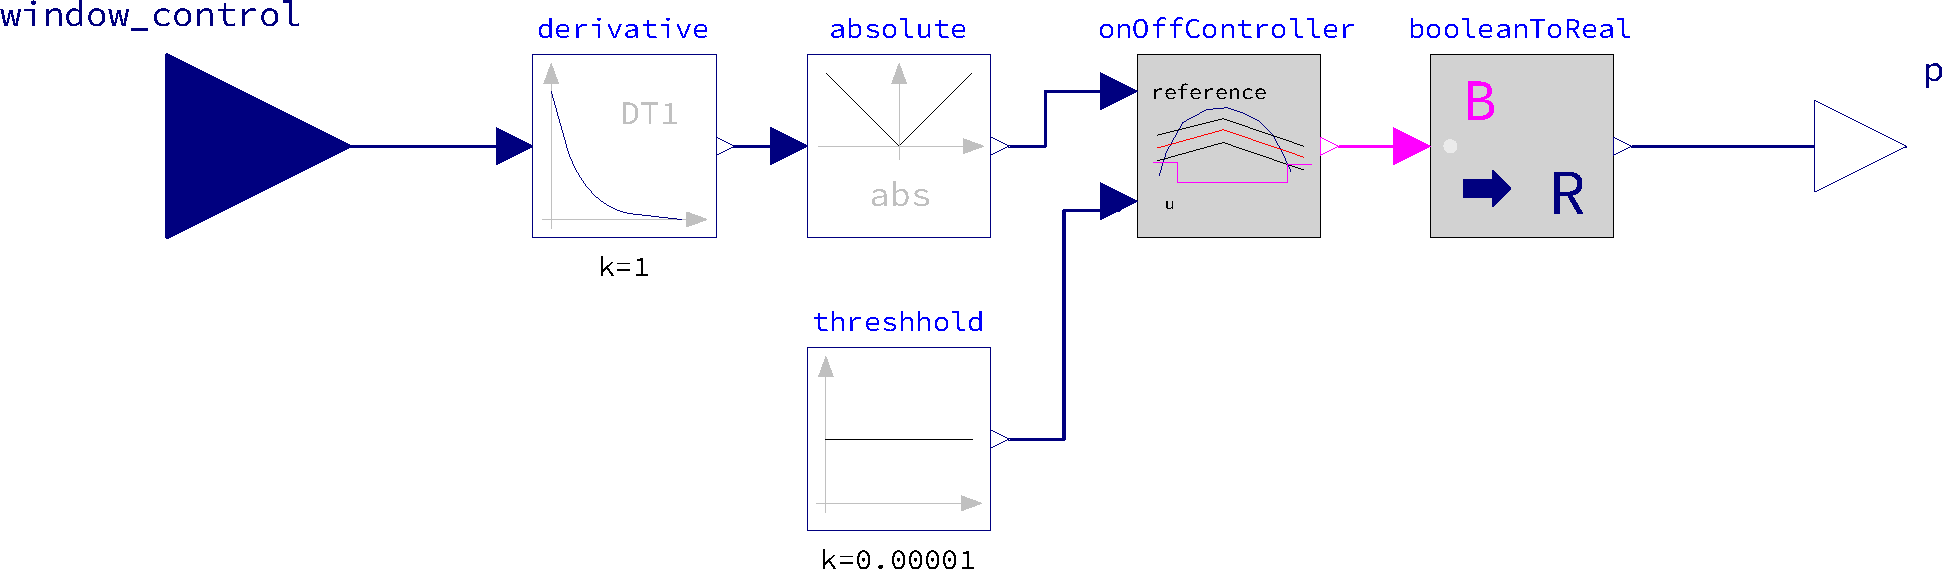
\includegraphics[width=\textwidth]{img/simulation/window-motors.pdf}
  \caption{The blocks modelling the energy consumption of the window control.}
  \label{fig:window-motors}
\end{figure}

\subsection{Water System}
As elaborated before in \ref{sub:power-arch}, the chosen pump has a power draw of \SI{4}{\kW}.
We want to ideally run it during the day to make use of the solar array.
So for the model it is assumed to be active at full power anytime the sun shines, to fill up the water tanks on the roof.
These then supply the irrigation system during nighttime.
When \lstinline{weaBus.HGloHor} -- the global horizontal radiation -- is greater zero, the pump is switched on.
It is argued that this is a sufficient pessimistic assumption to not underestimate the systems' power usage.

\begin{lstlisting}[basicstyle=\fontsize{9pt}{10.5pt}\ttfamily, caption={Model implementing the power requirements of the pump.}, label=lst:pump]
model pump
  Buildings.BoundaryConditions.WeatherData.Bus weaBus;
  Modelica.Blocks.Interfaces.RealOutput p;

equation
  if (weaBus.HGloHor > 0) then
    p = 4000;
  else
    p = 0;
  end if;

end pump;
\end{lstlisting}

So with this the \textit{Input} to this block is the weather data and the \textit{Output} is the power requirements for the water system.
Now that we have examined all the models part of the engineered system we have defined before, other implemented systems are discussed.
Starting with energy generation through a solar array.

\subsection{Photovoltaics}
For solar installations, there exists the 'pvSimple' model within the Buildings library.
This is implemented according to its documentation.
The systems' voltage is fixed at \SI{48}{\V}.
Azimuth and Tilt are set to 'south' and \SI{30}{\degree} respectively.
There might be more optimal values, this was however not further investigated.
The area of the solar array is set to be equal to the roof area of the building, which is \SI{1212}{\square\m}.
This value is calculated from the 3d-model \textcolor{Blue}{needs ref}.
Still two more parameters need to be defined.
First the fraction of the area which is covered by active panels is set to 0.8.
And the efficiency of the panels is assumed to be \SI{20}{\percent}.

\begin{figure}[htbp]
  \centering
  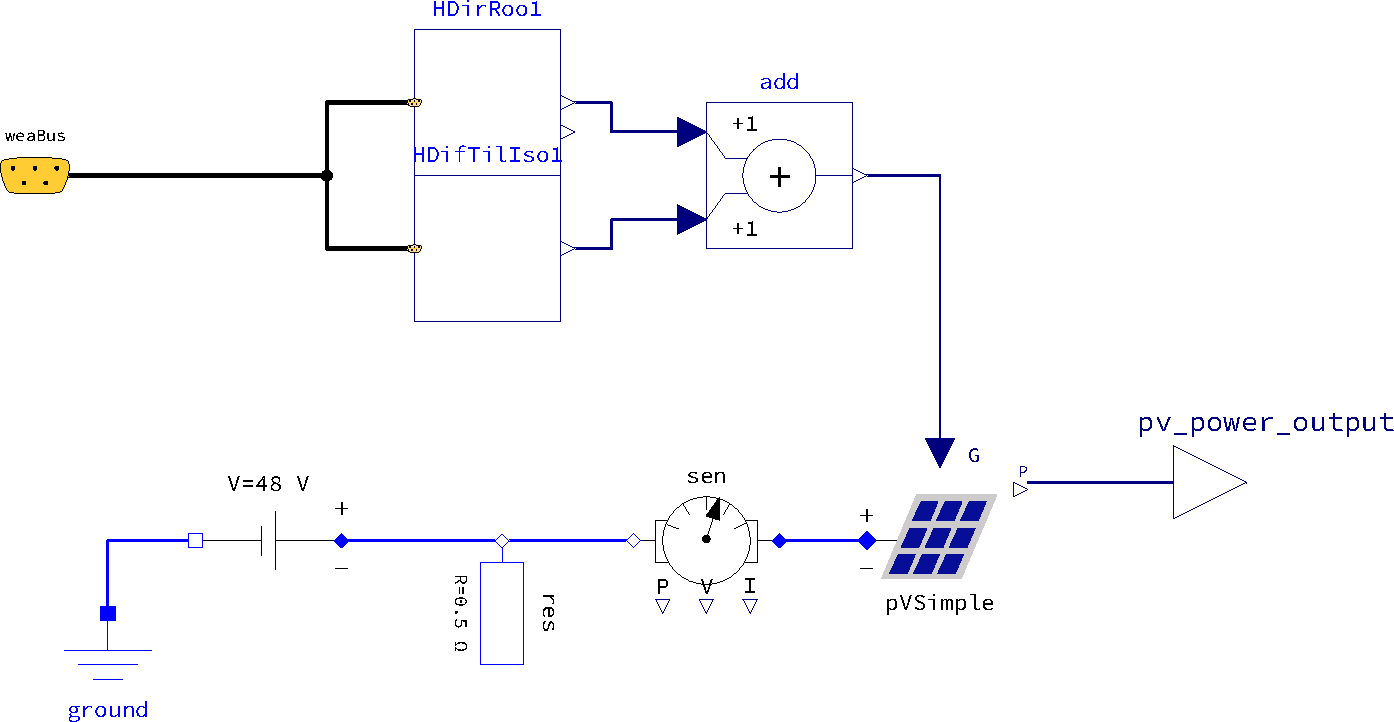
\includegraphics[width=\textwidth]{img/simulation/photovoltaik.pdf}
  \caption{The model for the solar array.}
  \label{fig:solar}
\end{figure}

\subsection{Physical Environment Model}

\textcolor{Blue}{Buildings.ThermalZones.ReducedOrder.RC.TwoElements for Radiation modelling}

\subsection{Building}

\subsection{City Environment}
The .eps file containing the needed information is taken from \textcolor{Blue}{needs ref}.

\subsection{Full system simulation}
With all the necessary building blocks introduced now, we can take a look at the final implementation.
The four farms are connected up to the building, the city environment and some analysis blocks.
They also take the power output of the solar array, as well as weather information as inputs.
The analysis blocks are colored consistent with the \ref{fig:simulation-architecture}.
This is shown in Figure \ref{fig:system}.

\begin{figure}[htbp]
  \centering
  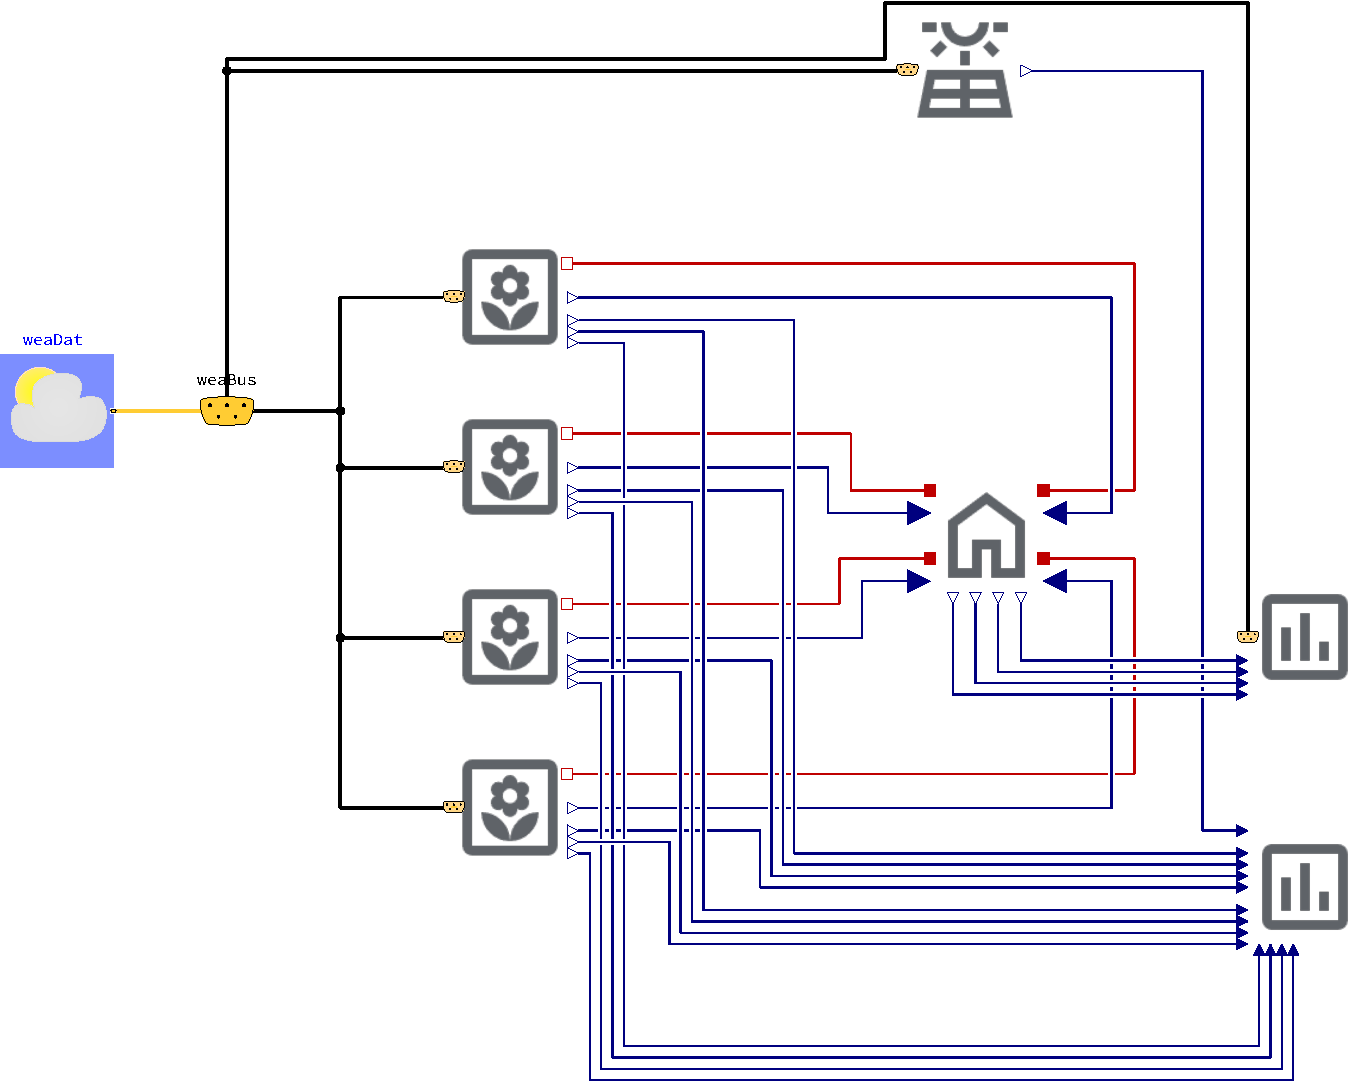
\includegraphics[width=\textwidth]{img/simulation/system.pdf}
  \caption{The full simulation.}
  \label{fig:system}
\end{figure}

\section{Analysis of Energy Use and Comparison with State of the Art}
\label{sec:sim-energy-and-comparison}

\section{Results}
\label{sec:simulation-results}
Insulation performance -- calculate average insulation value for the colder months.

Note that $\text{CO}_2$ concentrations are not dynamically calculated in the simulation and the humidity contribution from the plants is not considered.
The reason for this, is that the air volume component allowing for dynamic calculation led to frequent convergence errors not further investigated in this work.
The chosen value for $\text{CO}_2$ is 365 ppm, which is an average value for the atmosphere https://doi.org/10.1111/j.1365-3040.2007.01641.x.
For the \ac{vpd} calculation, humidity levels are taken from weather data and temperature from the farm air volume.

